\documentclass[10pt]{article}

\usepackage[utf8x]{inputenc}
\usepackage[english,italian]{babel}
\usepackage{graphicx}
\usepackage{booktabs}
\usepackage{caption}
\usepackage{textgreek}
\usepackage{tabularx}
\usepackage{amsmath,amssymb,stackengine}
\usepackage{authblk}
\usepackage{xcolor}


\usepackage{geometry} % to change the page dimensions
\geometry{a4paper} % or letterpaper (US) or a5paper or....
% \geometry{margin=2in} % for example, change the margins to 2 inches all round
% \geometry{landscape} % set up the page for landscape
%   read geometry.pdf for detailed page layout information

\usepackage{graphicx} % support the \includegraphics command and options

% \usepackage[parfill]{parskip} % Activate to begin paragraphs with an empty line rather than an indent

%%% PACKAGES
\usepackage{booktabs} % for much better looking tables
\usepackage{array} % for better arrays (eg matrices) in maths
\usepackage{paralist} % very flexible & customisable lists (eg. enumerate/itemize, etc.)
\usepackage{verbatim} % adds environment for commenting out blocks of text & for better verbatim
\usepackage{subfig} % make it possible to include more than one captioned figure/table in a single float
% These packages are all incorporated in the memoir class to one degree or another...

%%% HEADERS & FOOTERS
\usepackage{fancyhdr} % This should be set AFTER setting up the page geometry
\pagestyle{fancy} % options: empty , plain , fancy
\renewcommand{\headrulewidth}{0pt} % customise the layout...
\lhead{}\chead{}\rhead{}
\lfoot{}\cfoot{\thepage}\rfoot{}

\usepackage{sectsty}
\allsectionsfont{\sffamily\mdseries\upshape}

\usepackage[nottoc,notlof,notlot]{tocbibind}
\usepackage[titles,subfigure]{tocloft}

\renewcommand{\cftsecfont}{\rmfamily\mdseries\upshape}
\renewcommand{\cftsecpagefont}{\rmfamily\mdseries\upshape}
\newcommand*{\hham}{\mathcal{H}}
\newcommand*{\xx}{\vec{x}}
\newcommand*{\kk}{\vec{k}}
\newcommand*{\qq}{\vec{q}}
\newcommand*{\p}{\varphi}
\newcommand*{\zpart}{\mathcal{Z}}
\newcommand*{\w}{\Bigl}
\newcommand*{\lapint}{\int_{a-i\infty}^{a+i\infty}\frac{dz}{2\pi i}}

\definecolor{carmine}{rgb}{0.59, 0.0, 0.09}


\selectlanguage{english}

\title{On predator prey}

\author{Onofrio Mazzarisi}

\begin{document}

\selectlanguage{english}

\maketitle

\section{Non evolutionary scenario}
In this setting the model is as in the draft but without the evolution of costs functions.
The parameters are common to all the species and I report them here for reference:
resources consumption rate $\eta$, predators (on both levels) resource gain $\gamma$, reproduction threshold $d$,
primary resource regeneration rate $\lambda$ and a catch rate $q$ which represent the
probability that, when they meet, a predator catches a prey (it is the same for predators on both levels).
The linear dimension of the grid is denoted by $L$.

\subsection{Mean-field theory}
In order to understand the dynamics I formulated a mean-field theory for the problem
based on the observation that the relevant dynamical quantities are the internal resources of the agents.
I denote the internal resources of the $n$-th prey as $k^n_p$ and do the same
for first and secon level predators, respectively  $k^n_{\pi_1}$ and $k^n_{\pi_2}$ as in the draft.
The first step is to assume a well mixed population which allows to neglect spatial
structure and build the theory. In the following I derive the dynamical equations
for the total resources held by each species to leverage then on thier conservation at
stationarity in order to obtain expression for the densities of agents.

Let me start with the secondd level predators $\pi_2$, and consider the evolution of the internal resources
of a single agent (valid $\forall n$)
\begin{equation}
\label{eq:single_pi2}
\Delta_tk^n_{\pi_2} = -\eta + \gamma q P_{\pi_1},
\end{equation}
where $\Delta_tf \equiv f(t+\Delta t)-f(t)$, being $\Delta t$ a time step, and $P_{\pi_1}$
stands for the probabilty of the agent to encounter, in the gird cell where it moved,
{\it at least one} predator $\pi_1$. To obtain $P_{\pi_1}$ one can notice that
the probability of each of the $N_{\pi_1}$ first level predator to be found in
a given cell is $1/L^2$ (in force of the well mixing assumption). This implies that, detonig the density of
predators $\pi_1$ with $\rho_{\pi_1}=N_{\pi_1}/L^2$, the number random number $\xi$ of $\pi_1$
in a grid point is Poisson distributed
\begin{equation}
\mathcal P_{\rho_{\pi_1}}(\xi)=\frac{\rho_{\pi_1}^{\xi}}{\xi!}e^{-\rho_{\pi_1}},
\end{equation}
therefore $\mathcal P_{\rho_{\pi_1}}(0)=e^{-\rho_{\pi_1}}$ and $P_{\pi_1}= 1-e^{-\rho_{\pi_1}}$.
If I now sum over all the $\pi_2$ and divide by the grid size $L^2$, denoting $k_{\pi_2}=\sum_{n=1}^{N_{\pi_2}}k^n_{\pi_2}$, I obtain
\begin{equation}
\frac{\Delta_tk_{\pi_2}}{L^2} = -\eta\rho_{\pi_2}+ \gamma q (1-e^{-\rho_{\pi_1}})\rho_{\pi_2}.
\end{equation}

Before deriving the other two equations let me stress that it is possible to absorb
a parameter, $\eta$, in the definition of time (a sort of metabolic timescale)
and redefining all the other parameters as $\lambda/\eta\leftarrow\lambda$, $\gamma/\eta\leftarrow\gamma$,
$d/\eta\leftarrow d$ and $q/\eta\leftarrow q$ we can get rid of it (perfectly confirmed numerically).

The single agent equation for $\pi_1$ predators is {\it mutatis mutandis} the same as
Eq.~(\ref{eq:single_pi2})
\begin{equation}
\label{eq:single_pi1}
\Delta_tk^n_{\pi_2} = -1 + \gamma q (1-e^{-\rho_p}),
\end{equation}
where $(1-e^{-\rho_p})$ is the probability that at least one preys is present on the grid point
visited by the agent. A predator $\pi_1$, though, can be killed by predators $\pi_2$ and when this happen
the internal resources $k^n_{\pi_1}$ are lost; this has to be taken into account when looking at the
total resources $k_{\pi_1}$. I have
\begin{equation}
\frac{\Delta_tk_{\pi_1}}{L^2} = -\rho_{\pi_1}+ \gamma q (1-e^{-\rho_p})\rho_{\pi_1}-q(1-e^{-\rho_{\pi_2}})\frac{k_{\pi_1}}{L^2}\rho_{\pi_1},
\end{equation}
where $q(1-e^{-\rho_{\pi_2}})$ is the rate at which predators $\pi_1$ are killed. One can write
$k_{\pi_1}/L^2=\rho_{\pi_1}k_{\pi_1}/N_{\pi_1}=\rho_{\pi_1}d\alpha_{\pi_1}$ assuming that at stationarity
the average amount of resources held by a single $\pi_1$ is a fraction $\alpha_{\pi_1}$ of the reproduciton
threshold $d$ and arrive at
\begin{equation}
\frac{\Delta_tk_{\pi_1}}{L^2} = -\rho_{\pi_1}+ \gamma q (1-e^{-\rho_p})\rho_{\pi_1}-qd\alpha_{\pi_1}(1-e^{-\rho_{\pi_2}})\rho_{\pi_1}.
\end{equation}
Preys share the resources found on the ground, therefore for the $n$-th prey one can write
\begin{equation}
\Delta_tk^n_p = -1 + \frac{\lambda}{\rho_p},
\end{equation}
and thus, with obvious notation,
\begin{equation}
\frac{\Delta_tk_p}{L^2} = -\rho_p +\lambda-qd\alpha_p(1-e^{-\rho_{\pi_1}})\rho_p.
\end{equation}
It is interesting that the amount of resources acquired by the totality of the preys (per unit area)
is exactly $\lambda$.
An other way to recognise this would be to think directly in terms of total population.
The average amount of resources in a grid point can be estimated as $\lambda/(1-e^{-\rho_p})$,
because for every time-step that preys don't visit the point it increases by $\lambda$.
Therefore the total amount of resources (per unit area) acquired by the preys is this number
multiplied by the fraction of occupied grid points, which is $(1-e^{-\rho_p})$.

Collecting everything, at stationarity, I have
\begin{align}
0 &= -\rho_{\pi_2}+ \gamma q (1-e^{-\rho_{\pi_1}})\rho_{\pi_2}, \nonumber \\
0 &= -\rho_{\pi_1}+ \gamma q (1-e^{-\rho_p})\rho_{\pi_1}-qd\alpha_{\pi_1}(1-e^{-\rho_{\pi_2}})\rho_{\pi_1}, \\
0 &= -\rho_p +\lambda-qd\alpha_p(1-e^{-\rho_{\pi_1}})\rho_p. \nonumber
\end{align}
Notice that in all three equations $d$ and $\gamma$ always appears multiplied by $q$, and the latter
is never present alone, thus we can redefine $\gamma q\leftarrow \gamma$ and $dq\leftarrow d$ and absorb it
(perfect numerical check).
Finally the equations for the densities read
\begin{align}
\label{eq:three-levels}
\rho_p &=\frac{\lambda }{1+\alpha_p d /\gamma} , \nonumber \\
\rho_{\pi_1} &= \ln \left(\frac{\gamma}{\gamma -1}\right), \\
\rho_{\pi_2} &= \ln \left\{\frac{1+ \alpha_{\pi_1}d -\gamma  \left[1-e^{-\lambda / (1+\alpha_p d /\gamma)}\right]}{\alpha_{\pi_1}d} \right\}. \nonumber
\end{align}
An interesting observation from the simulation is that the fractions $\alpha_p\simeq 2/3 \simeq\alpha_{\pi_1}$
robustly w.r.t. the variation of the parameters. This is nice and intuitive because at stationarity one
expects that $p$ and $\pi_1$, having both to support an upper trophic level
(the first $\pi_1$ and the second $\pi_2$),
indeed have an average amount of internal resources which is between the reproduction
threshold $d$ and $d/2$ (the initial amount of the progeny). The only parameters in the game remain $d$ and $\gamma$,
a part of course form the indipendent variable $\lambda$.
\begin{center}
\begin{figure}[h]
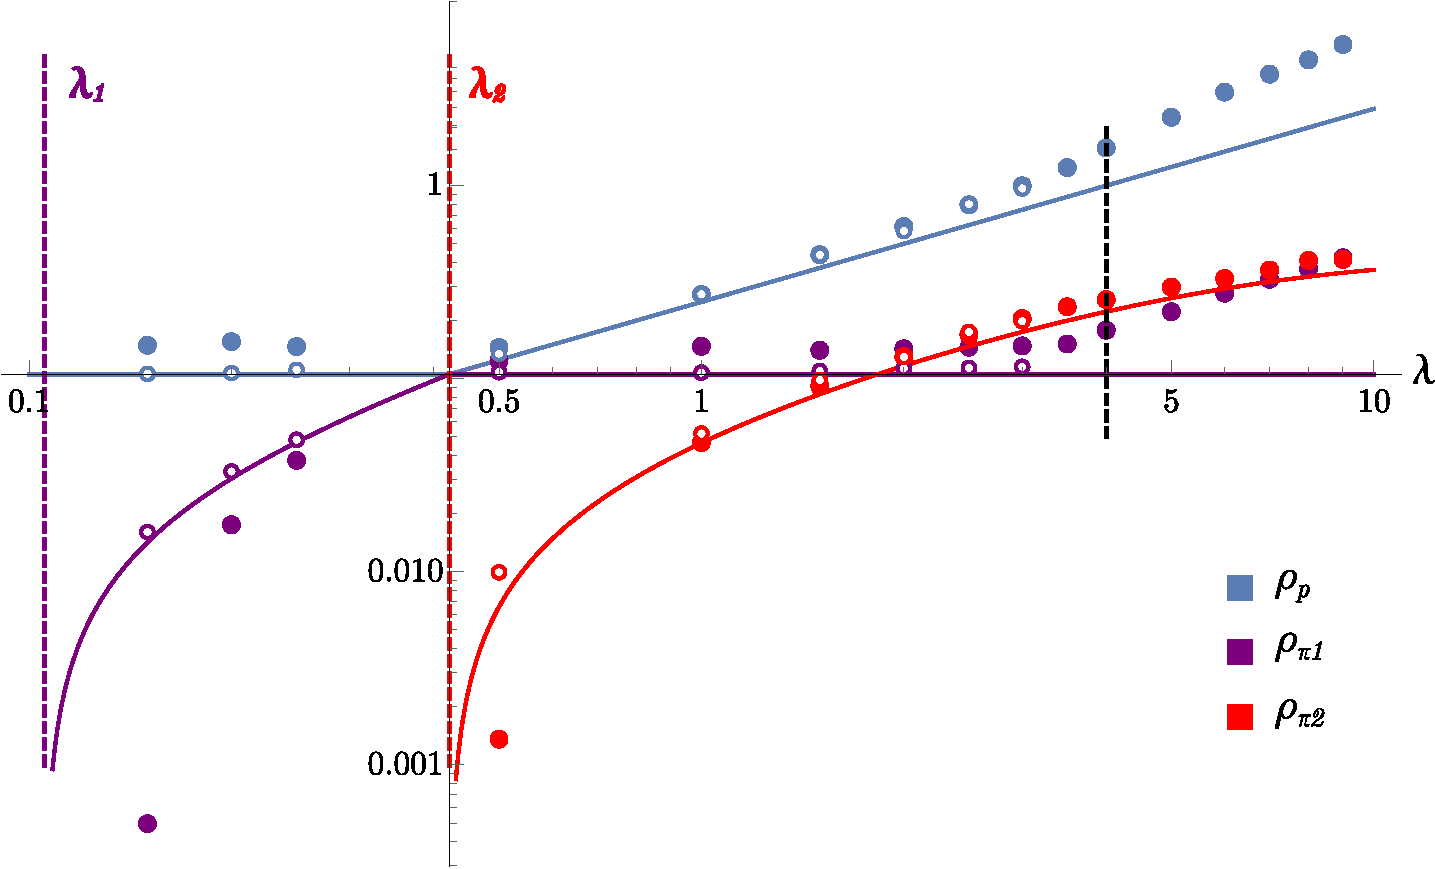
\includegraphics[width=1\linewidth]{sim2.pdf}
\caption{Prey density $\rho_p$ (blue), first level predator density $\rho_{\pi_1}$ (purple) and second level
predator density $\rho_{\pi_2}$ (red) are plotted against $\lambda$ for fixed $d=40$ and $\gamma=10$.
Solid lines represent mean-field theory predictions from Eqs.~(\ref{eq:three-levels},\ref{eq:two-levels}).
Purple and red dashed vertical lines stands respectively for $\lambda_1$ (Eq.~(\ref{eq:lambda1})) and $\lambda_2$
(Eq.~(\ref{eq:lambda2})). Solid dots correspond to simulations with Moore connectivity while empty ones
to a fully connected graph. The values are time averages from time 300 to time 3000 or form time 500 to time 5000
(where a time step consist of the movement of every agent in the grid) and $L$ varies from 30 to 150.
Both choices (time and size) are such that, at the given value of $\lambda$
a stable solution is attained and the system is there for enough time to have an acceptable statistics.}
\label{pic:simulations}
\end{figure}
\end{center}
In Fig.~\ref{pic:simulations} are reported results of simulations (see caption for details) and compared with
the mean field theory for $d=40$ and $\gamma=10$.

The red dashed vertical line in Fig.~\ref{pic:simulations} correspond to the point
\begin{equation}
\label{eq:lambda2}
\lambda_2 = \left(\frac{d\alpha_p}{\gamma}+1\right)\ln\left(\frac{\gamma}{\gamma-1}\right) ,
\end{equation}
obtained using the last of Eqs.~(\ref{eq:three-levels}),
below which no positive solution for $\rho_{\pi_2}$ exists and the system reduces to a two level
food web. In this regime, using the same arguments as above, the mean-field equations for preys and
predators $\pi_1$ reads
\begin{align}
\label{eq:two-levels}
\rho_p &= \ln \left(\frac{\gamma}{\gamma -1}\right) , \nonumber \\
\rho_{\pi_1} &= \ln\left[\frac{\ln\left(\frac{\gamma}{\gamma-1}\right)\alpha_p d}{\ln\left(\frac{\gamma}{\gamma-1}\right)(\alpha_p d -1)+\lambda}\right].
\end{align}
The value of $\lambda$ below which also the population of $\pi_1$ can not be supported
, i.e. when the second of Eqs.~(\ref{eq:two-levels}) becomes negative, is
\begin{equation}
\label{eq:lambda1}
\lambda_1= \ln \left(\frac{\gamma}{\gamma -1}\right),
\end{equation}
represented by the purple dashed vertical line in Fig.~\ref{pic:simulations}.
The phase transitions observed in the simulations (at least in the non evolutionary setting)
are therefore perfectly described by the mean-field theory.

Let me discuss now the break down of the mean-field theory for high value of $\lambda$.
More precisely this happens, robustly with respect ot variations of $d$ and $\gamma$,
when $\rho_p>1$, therefore, form the first of Eqs.~(\ref{eq:three-levels}), at
\begin{equation}
\lambda^c=1+\frac{\alpha_p d}{\gamma},
\end{equation}
which is represented by the black dashed vertical line in Fig.~\ref{pic:simulations}.
Here, numerically, happens that for a fully connected graph, the system does not have a stable
stationary solution but a limit cycle (yet to be characterized) appears. Curiously
enough in the case of Moore connectivity stable solutions exists (better simulations needed though
to completely confirm this) but they dviate from the
mean field predicion and an allometric relation between $\rho_p$ and $\rho_{\pi_1}$ sets in
with roughly $\rho_{\pi_1}\sim\rho_p^{3/4}$. I have some ideas on why this happens but are too
speculative for now, a discussion is in order. I want just to mention that this "strange" deviation
appears for values of the parameter $\lambda$ in a weird regime, meaning in a regime where the
density of prey exceeds 1, and can be questioned that such regime is of interest in understanding
realistic scenarios.

A part from this last point, which is though of the highest importance to clarify,
the mean-field presented completely characterize the model and exclude
allometric relation for reasonable (?) values of the parameters.

\begin{equation}
  prova2
\end{equation}

\bibliography{Bib/library.bib}

\bibliographystyle{unsrt}

\end{document}
